\chapter{From OS to API}
Most of the fuzzers we have seen so far are focused on low-level fuzzing. They are fuzzing the syscalls, image formats, web browsers, etc. This is utterly understandable since fuzzers are best at exposing memory bugs like use-after-frees, all kinds of buffer overflow, or uninitialized memory \cite{chang2017oss}. These types of bugs naturally occur in memory unsafe languages like C or C++. The main use of memory unsafe languages is in programs that are meant to be performant or interact with the underlining system. Thus, we may see them used in system programming and GUI applications.

However, the global trend is to move away from GUI applications and offer all services via the web. We can see it, for example, in office suits. Microsoft is now offering the entire office suite online. Furthermore, Google offers the office suite only online. The same goes for email clients, chat applications, video players, text editors, and many more.

To secure these online applications, we need to be able to fuzz the web services. Web services, nonetheless, are not as simple as a single application or binary. They may consist of several other services in the background. One of the prevalent ways to organize web services is to use the microservice architecture, which we describe in the next section.

\section{What are microservices}
Microservice architecture is a way to organize multiple loosely coupled services. Those services are typically lightweight and try to follow the Unix philosophy of doing one thing and doing it well. What is more essential for us, is that they communicate mostly via technology-agnostic protocols \cite{nadareishvili2016microservice}. One of those protocols is HTTP. Moreover, the services often use representational state transfer (REST) architectural style. Let us explore the characteristics of such an application in more depth.

\section{What is REST and RESTfull}
The representational state transfer or simply REST is a set of architectural principles to follow when creating a web service. Furthermore, applications that follow the REST guides are said to be RESTfull. Alex Rodrigues in his article about RESTfull web services summed up the principles in four straightforward points \cite{rodriguez2008restful}.

\begin{itemize}
  \item Use HTTP methods explicitly
  \item Be stateless
  \item Expose directory structure-like URIs
  \item Transfer XML, JavaScript Object Notation (JSON), or both
\end{itemize}

\paragraph{}
\textbf{Using HTTP methods explicitly} means to adhere to the one-to-one mapping between HTTP methods and CRUD operations. The CRUD operations are create, read, update and delete. The GET method should be used to retrieve a resouce and is supposed to cause no side effects. On the other hand, the POST method is designated for the creation of a resource on the server. To update the resource, one ought to use the PUT method, and finally, to delete the resource, the DELETE method should be used.

\paragraph{}
\textbf{To be stateless} the client and server need to send complete and independent requests. By sending complete and independent requests servers can take an advantage of load-balancing or forwarding the payload to other services for further processing. An ilustrative example is the case of pagination. If the communication would be stateful (as shown in the figure \ref{fig:Stateful request example}), the server would need to cache the current page of the client. That would mean that only a single server would be able to be deployed to hold the state. On the other side, stateless request (as shown in the figure \ref{fig:Stateless request example}) enables the server to load-balance easily.

\begin{figure}[h]
  \begin{subfigure}{}
    \begin{minipage}{0.5\textwidth}
      \begin{minted}{HTTP}
GET /books HTTP/1.1
Host: server
Content-Type: application/json

{"page": 3}
      \end{minted}
      \caption{Stateless request example}
      \label{fig:Stateless request example}
    \end{minipage}
  \end{subfigure}
  \begin{subfigure}{}
    \begin{minipage}{0.5\textwidth}
      \begin{minted}{HTTP}
GET /books?nextpage=true HTTP/1.1
Host: server
      \end{minted}
      \caption{Stateful request example}
      \label{fig:Stateful request example}
    \end{minipage}
  \end{subfigure}
\end{figure}

\paragraph{}
The third principle of REST design is \textbf{exposing directory structure-like URIs}. URIs in REST architecture should be intuitive, easy to guess, and follow a tree-like hierarchy. GitHub API exposes URIs in a directory structure-like format. For example, to create a new repository in an organization, one would make a POST request to this URI: \texttt{/repos/{owner}/{repo}/projects}. Moreover, the directory structure-like URIs are also acting as a self-documentation of the API. In addition, adherence to this principle makes it easier to swap underlining technology because directory structure-like URIs do not expose the scripting technology file extensions like \texttt{.php} or \texttt{.asp}.

\paragraph{}
The final principle is to \textbf{transfer XML, JavaScript Object Notation (JSON), or both.} Those formats have the advantage of being standardized, simple, and human-readable. Most programing languages have libraries for parsing the formats.

\paragraph{}
To help us model and document the APIs more precisely, OpenAPI specifications can be used. We will describe it in more detail in the next section since we will refer to it in existing fuzzers and our implementation.


\section{What is OpenAPI specification}
\label{sec:openapi}
OpenAPI specification is a way to describes and document an API. Moreover, it is described in a  machine-readable format (in YAML and JSON). In addition to a machine-readable format, an interactive UI can be generated from the specification as well.

Two major versions of OpenAPI specification are currently used. The older one is version 2, previously known as Swagger. The newer one which was standardized in 2016 and become overseen by the OpenAPI Initiative \cite{openapi2020main} later is version 3. There are not so many differences between those versions, however, version 3 included breaking changes which means that a new major version needed to be issued. Furthermore, there are also converters between the two versions. We will now focus on the newer one as its gaining more acceptance in the ecosystem. Version 3 with generated UI can be seen in figure \ref{fig:openapi-specification}.

\begin{figure}[h]
  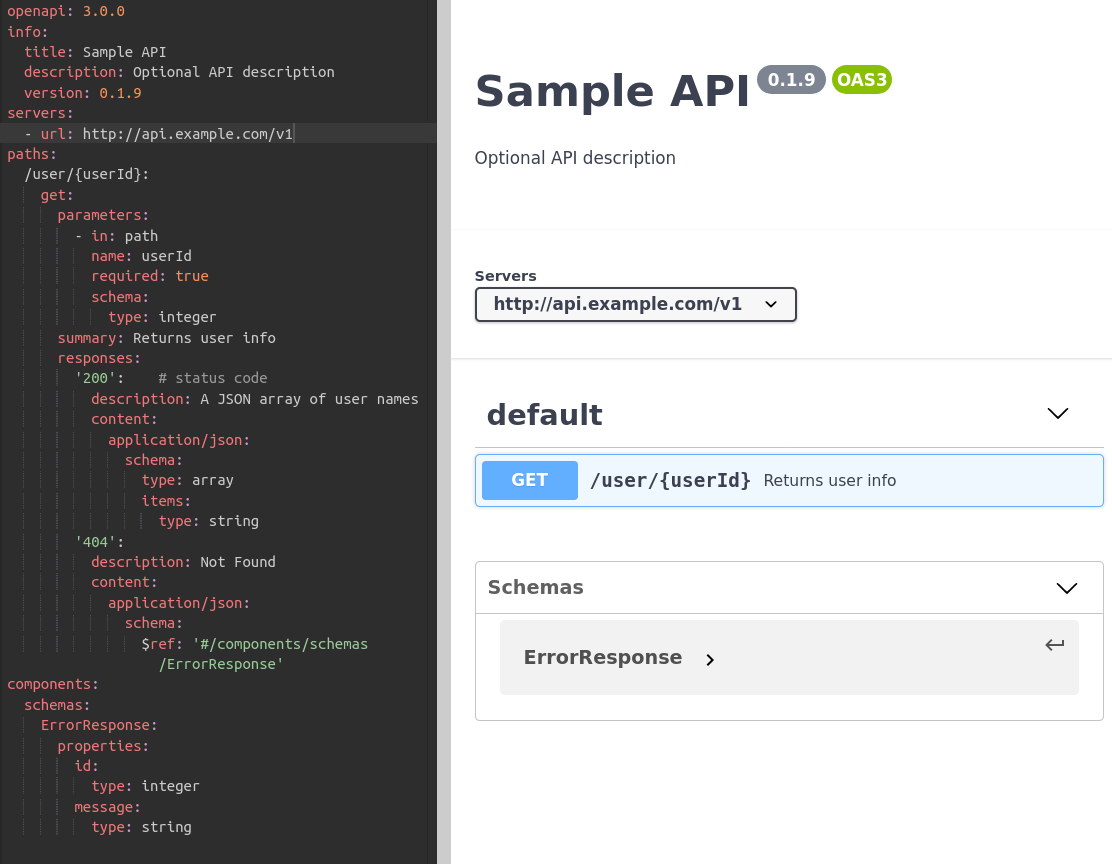
\includegraphics[width=\textwidth]{openapi-specification}
  \caption{OpenAPI specification in YAML format and generated UI}
  \label{fig:openapi-specification}
\end{figure}

Let us have a look at the structure of OpenAPI specification and its separate fields to gain better knowledge about provided information. We will focus on context of fuzzing when describing it since it will be instrumental in subseqent chapters where we will take a look at existing work and implementation of our own fuzzer.

\subsection{What OpenAPI provides}
As we mentioned before, the OpenAPI specification is in JSON or YAML format. We will now traverse the structure and analyze \textit{keys} or \textit{sections} that may be used when fuzzing.

Every OpenAPI specification needs to have a \textbf{openapi} \textit{key} of type string that describes the version of the specification. Moreover, the key must follow the semantic versioning system.

Another \textit{key} in the specification is \textbf{info} which provides metadata about the API mainly. The info is as well a required section and it can contain a license, title, or version \cite{openapi2020github}.

The next section that may be present in the specification is \textbf{servers}. This section contains a list of URLs from which the API can be accessed. The servers section provides also a key-value mapping between URL variables that can be used for example for versioning as can be seen in figure \ref{fig:Server definition with variables}. However, since this definition is not required, numerous APIs do not use it and include the URL in the description of other sections. Moreover, the variable mapping is also used only occasionally. This inconsistency in usage makes the server definition not suitable for machine processing and therefore for fuzzing.

\begin{figure}[h]
  \begin{minted}{YAML}
servers:
- url: https://server.com/{basePath}
  variables:
    basePath:
      default: v2
  \end{minted}
  \caption{Server definition with variables example}
  \label{fig:Server definition with variables}
\end{figure}

The most informative and therefore most essential section of the OpenAPI specification is \textbf{paths}. The path section consists of a list of path objects definitions, where each definition describes one resource (URI path). Here we may notice the interconnection between the REST design strategy and the OpenAPI specification. For each resource, there are defined methods that correspond to the CRUD operations for the manipulation of the resource. Every method of a resource describes in great detail how the request to the described resource should look like. It defines the request body, its content type, structure, and types. Similarly, it defines the parameters. From the parameter's definition, we determine where they are located, whether it is a path, headers, cookies or query parameters. What is their structure, types, and if they are required. In addition to possible inputs of the resource, the method definition states the possible outputs as well - responses. The definition of responses supplies list of response objects. Every response object defines a HTTP status code, headers, and content that can be received as a response from particular resource-method pair. The content object is rather akin to the request body object. It defines the content type, structure, and types of the fields in the structure as well.

\label{subsec:components}
As you know APIs reuse many things and the same holds true for their descriptions. For instance, the structure of the error message may be the same for every resource. Another example can be listing objects and getting a single one. The structure of responses or even requests might be rather alike. One can imagine how tedious and error-prone would it be to write the same definitions to numerous resources. For this particular reason OpenAPI specification defines a section called \textbf{components}. In the components section, user may define structures, as a single point of truth, that can be subsequently referenced in other sections. An example can be seen in figure \ref{fig:openapi-specification} where the \texttt{ErrorResponse} object is defined in components section and referenced from response object in \texttt{/user/\{userID\}} resource.

The last top-level section that we will explore is \textbf{security} section. This section illustrates which authorization schemes the API uses. The security scheme consists of a type, for instance, apiKey, HTTP basic authentication, oauth2, openIdConnect or mutualTLS, name, its location in the request, and other information based on the scheme type. The authorization scheme can be then applied per resource-method pair or to the whole API.


\paragraph{}
Now that we have a deeper understanding of what OpenAPI specification provides, we can have a look at the existing work in the fields of fuzzing web services. We will see if or how the OpenAPI specification was used in the existing work and in later chapters we will detail how it can help us to implement a \emph{smart} fuzzer.
